%%%%%%%%%%%%%%%%%%%%%%%%%%%%%%%%%%%%%%%%%
% Simple Sectioned Essay Template
% LaTeX Template
%
% This template has been downloaded from:
% http://www.latextemplates.com
%
% Note:
% The \lipsum[#] commands throughout this template generate dummy text
% to fill the template out. These commands should all be removed when 
% writing essay content.
%
%%%%%%%%%%%%%%%%%%%%%%%%%%%%%%%%%%%%%%%%%

%----------------------------------------------------------------------------------------
%	PACKAGES AND OTHER DOCUMENT CONFIGURATIONS
%----------------------------------------------------------------------------------------

\documentclass[12pt]{article} % Default font size is 12pt, it can be changed here


 
\usepackage{geometry} % Required to change the page size to A4
\geometry{a4paper} % Set the page size to be A4 as opposed to the default US Letter

\usepackage{graphicx} % Required for including pictures

\usepackage{float} % Allows putting an [H] in \begin{figure} to specify the exact location of the figure
\usepackage{wrapfig} % Allows in-line images such as the example fish picture

\linespread{1.2} % Line spacing

%\setlength\parindent{0pt} % Uncomment to remove all indentation from paragraphs

\graphicspath{{./Pictures/}} % Specifies the directory where pictures are stored

\usepackage{listings}
\usepackage{tabulary}

\begin{document}

\setcounter{secnumdepth}{3}
\setcounter{tocdepth}{3}

%----------------------------------------------------------------------------------------
%	TITLE PAGE
%----------------------------------------------------------------------------------------

\begin{titlepage}

\newcommand{\HRule}{\rule{\linewidth}{0.5mm}} % Defines a new command for the horizontal lines, change thickness here

\center % Center everything on the page

\textsc{\LARGE CERN IT-SDC}\\[1.5cm] % Name of your university/college
%\textsc{\Large Major Heading}\\[0.5cm] % Major heading such as course name
%\textsc{\large Minor Heading}\\[0.5cm] % Minor heading such as course title

\HRule \\[0.4cm]
{ \huge \bfseries XrdHTTP}\\[0.4cm] % Title of your document
\textsc{\Large An HTTP/WebDAV plugin for the Xrootd framework}\\[0.5cm]
\HRule \\[1.5cm]

\begin{minipage}{0.4\textwidth}
\begin{flushleft} \large
\emph{Author:}\\
Fabrizio \textsc{Furano} \\ % Your name\\
\end{flushleft}
\end{minipage}
%~
%\begin{minipage}{0.4\textwidth}
%\begin{flushright} \large
%\emph{Supervisor:} \\
%Dr. James \textsc{Smith} % Supervisor's Name
%\end{flushright}
%\end{minipage}\\[4cm]


%{\large \today}\\[3cm] % Date, change the \today to a set date if you want to be precise
{\large August 08, 2013}\\[3cm] % Date, change the \today to a set date if you want to be precise
%\includegraphics{Logo}\\[1cm] % Include a department/university logo - this will require the graphicx package


\vfill % Fill the rest of the page with whitespace

\end{titlepage}

%----------------------------------------------------------------------------------------
%	TABLE OF CONTENTS
%----------------------------------------------------------------------------------------

\tableofcontents % Include a table of contents

\newpage % Begins the essay on a new page instead of on the same page as the table of contents 





\begin{abstract}
This document describes our HTTP/WebDAV interface to the Xrootd framework. Deploying this plugin in an already existing deployment of Xrootd will provide high performance HTTP and WebDAV functionalities that are compatible with the Grid usage and with the LCGDM HTTP headers for replica management. The technical choices that led to the design of the plugin have been mostly pragmatic "least efforts" that wanted to privilege robustness, performance and deployment simplicity. Due to the technical nature of this document, we summarize relevant parts of requirements, specifications and design topics that are related to the objective. These considerations come from several discussions and interactions with Markus Shulz, Dirk Duellmann, Oliver Keeble and Andrew Hanushevsky, plus an older working proof-of-concept prototype.

\end{abstract}






\section{Introduction and goals}
The objective of the project is to make an xrootd-based storage endpoint able to support:

\begin{itemize}

\item HTTP/HTTPS data access functionalities, including authentication \footnote{\label{note1_authn}The meaning of 'authentication' here is the secure extraction of the user’s credentials from the secure connection. These credentials are then passed to the regular Xrootd authorization scheme chosen by the system administrator.}

\subitem this includes the EMI and IT/GT conventions on HTTP/DAV described here: https://svnweb.cern.ch/trac/lcgdm/wiki/Dpm/WebDAV

\item basic WebDAV metadata functionalities, including authentication \footnotemark[\ref{note1_authn}]

\subitem plus a small selection taken from the EMI and IT/GT extensions to DAV, for HEP data management https://svnweb.cern.ch/trac/lcgdm/wiki/Dpm/WebDAV. In particular file and replica listing and stat operations on files.
\end{itemize}

 One of the goals of this project is to let the regular components of the xrootd framework perform their normal authorization steps, once the appropriate information is properly passed to them. This can also be seen as a way to:

\begin{itemize}
 \item avoid having to reimplement code that performs the authorization
 \item avoid having to adapt/import/wrap code that performs the authorization
 \item reduce to a minimum the configuration steps that the system administrators will have to follow in order to enable HTTP/DAV-based data access in their pre-existing storage clusters.
\end{itemize}

 Another goal of the project is to open the possibility of using mainstream Web clients to interact with an Xrootd cluster, within the limits of the sophistication and completeness of the implementation of these clients.

\section{Rationale}

Easing the wider adoption of the HTTP protocol in HEP data access. There is substantial consensus in the HEP community about exploring the usage of the HTTP protocol for certain tasks that are related to analyzing or managing data.\\
At the same time the storage systems that are set up often need to support a matching set of access protocols, to allow simpler and more performant access from the client applications. This XrdHTTP effort is aimed at making it possible for a storage site that is based on the xrootd technology to join a growing ecosystem of applications that is based on HTTP. One way we foster the HTTP ecosystem is by contributing the components that fill the gaps between the functionalities that are needed by the World Wide Web browsing and the functionalities that are needed by data analysis applications.\\
HTTP is a very flexible protocol, and, whenever possible we want to help other development teams in harmonizing their data access solutions based on the HTTP protocol, following the conventions and extensions proposed by the EMI storage elements like DPM.

In this case, we want to make it possible for a storage cluster using the Xrootd framework to join a computing model that needs HTTP access or a Storage Federation based on the HTTP and WebDAV protocols.

\begin{figure}
  \begin{center}
    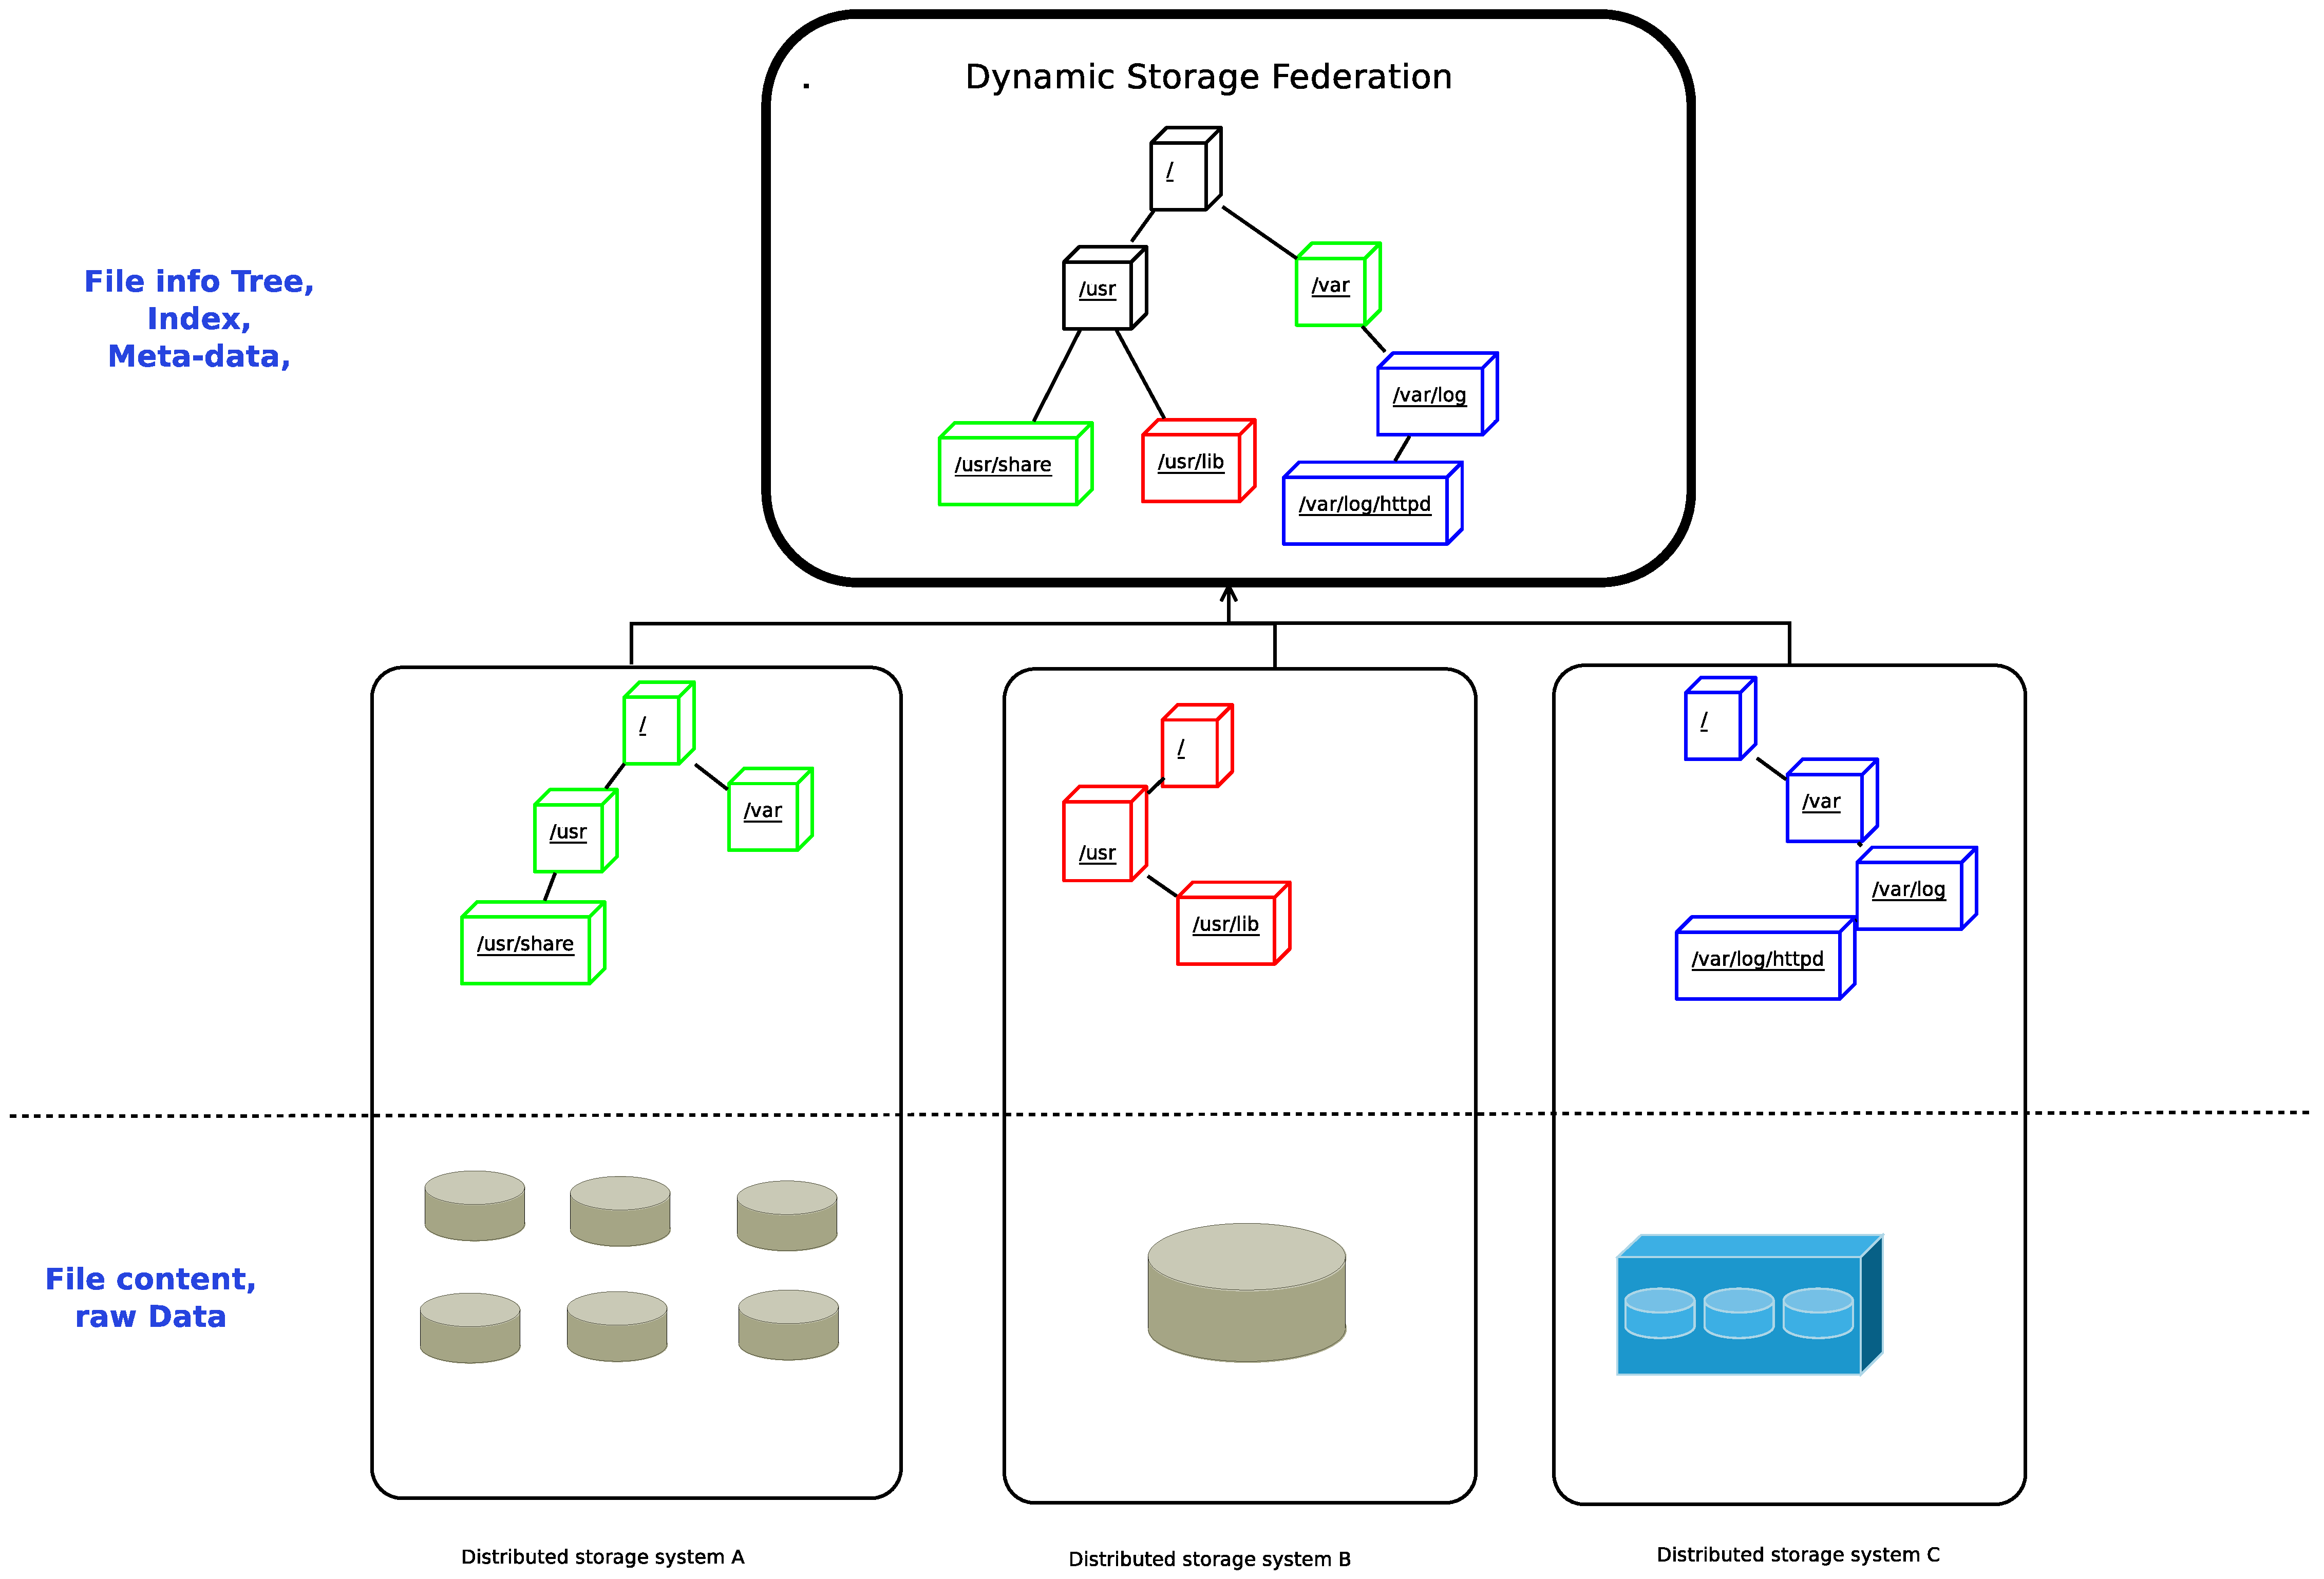
\includegraphics[width=28pc]{diagram-principle.eps}
  \end{center}
  \caption{\label{fig_mergenamespace}An example of how a storage federation would look like.}
\end{figure}

\subsection{Clustering of storage resources, federations}

XrdHTTP belongs to the categories of software systems whose goal is to cluster storage resources and make them available to data processing clients as if they were a unique system. Many other projects have analogous functionalities, in the Scientific community (e.g. DPM, dCache, iRODS) or in the market.

Some of these products, like  DPM, dCache and XRootd work by managing and distributing data across mountpoints that are spread through many servers. Clients that want to access the repository are redirected to the best machine according to various criteria, typically given by some clustering algorithm. There are different clustering techniques using various technologies (p2p-like, database, hashes, ...) and the goal of such systems is always to hide to the users doing analysis and data access the complexity of managing site resources
for repositories that are too big for a single server to be able to sustain the load that the clients would generate.\\

The sysadmins use these systems to organize the resources of a site and give a coherent service.
From the technical point of view, the goal is to hide to the users doing analysis and data access the complexity linked to the ``where is my file problem''. The central systems that schedule analysis jobs to be submitted, or the users themselves do not need to deal with details that are internal to the site (e.g. the names of the mount points, which can vary); they need to interact with a coherent storage service that is offered and administered by the site.\\

Very similar, or the same clustering techniques can be applied to cluster together sites into a larger entity that is informally called \textit{storage federation}. The emphasis here is on this being the same concept of clustering local disk arrays and mount points, extended to be able to work through a Wide Area Network, to cluster sites. Examples of these are LFC, the same Xrootd clustering (named Xrootd federations in this case), and the Dynamic Federations for HTTP or catalogue databases.\\

In addition to LFC and native Xrootd storage federations, an Xrootd storage cluster using the XrdHTTP plugin can be federated in an HTTP/WebDAV storage federation with no additional configuration effort, provided that its HTTP port is accessible from the Internet.

\section{Technical overview}

The Xrootd framework is a sophisticated plugin loading architecture, where the exposed functionalities can be defined through the so-called \textit{Protocol plugins}. The Protocol plugins are technically subclasses of the class \textit{XrdProtocol}, from which they inherit the basic behavior.
Instances of the \textit{XrdProtocol} plugins must implement:
\begin{itemize}
\item the very basic methods of the \textit{XrdProtocol} class, and all the purely virtual methods
\item the interface of the protocol, that is how it looks like in the communication channel that it is assigned to in order to serve clients (a TCP socket)
\item the actions that are associated to the various requests of the protocol.
\end{itemize}

The XrdHTTP plugin is only one plugin, in the form of a shared library. No instrumentations of the server machine, scripts or cronjobs are needed to make it work. In order for it to be effective, it has to be loaded by redirectors and data servers of an xrootd cluster to be enabled to serving HTTP. What follows is a list of the dependencies of the XrdHTTP plugin towards external packages. One of the goals of this design is to minimize the effort starting from minimizing this set of dependencies.\\

\begin{itemize}
 \item VOMS libraries $>=$ v2.0.8
 \item openSSL libraries $>=$ v0.9.8k
 \item the xrootd framework $>=$ (the main  requirement is the availability of the \textit{Protocol Bridge} functionality.)
 \item libXML
\end{itemize}


\subsection{Security}

XrdHTTP natively supports the following authentication methods:

\begin{itemize}
\item regular HTTPS clients, like browsers
\item X509 certificates as method of authentication
\subitem X509 RFC proxy certificates
\subitem X509 Globus proxy certificates, with VOMS extensions
\end{itemize}

The features that are related to VOMS and proxy certificates are supported through the usage of the \textit{libvoms2} library, through a security extractor plugin called XrdHttpVOMS, whose source code is part of the XrdHTTP. For these features to be available, this plugin has to be loaded by XrdHTTP.

For further technical details about how \textit{libvoms2} works, we refer to the \textit{libvoms2} documentation.

\subsection{Notes on mainstream clients}

To the best of our knowledge, all the mainstream HTTP and WebDAV clients that are available in the Linux distributions work and are supposed to work. At the same time, the standard misses a specification of the minimum feature set for a product to be declared standard. This uneven features support in the mainstream clients is more often affecting areas like:
\begin{itemize}
\item X509 authentication
\item Grid proxy authentication
\item Redirection on requests different than GET
\end{itemize}
When looking for an HTTP/WebDAV client that supports the whole feature set that is supported by XrdHTTP, we advice the reader to use the \textit{Davix} client from the Fedora and EPEL repositories.

\subsection{Runtime transparency}

One of the main technical features of XrdHTTP is the possibility of running the HTTP protocol on the same port that is assigned to the Xrootd protocol. Both protocols will work, and the clients will be automatically detected and properly handled. System administrators always can choose a different port for HTTP/HTTPS, for example to make it easier to discriminate the traffic from systems like Lemon or Nagios.

Internally, such detection works as follows. When the framework detects an incoming connection, it can ask to all the protocol plugins that were assigned to that port if they think that they want that connection for them (generally by peeking the first bytes sent by the client, which contain recognizable sequences of bytes). Depending on the answers, the framework then assigns the connection to one of them.
 
The goal of this is to allow the installation of the HTTP service without modifying any TCP-related rule or tunings that sites may have.
Although the feature is simple, its implementation details and the last answer about its feasibility depend also on the recognizability of the first bytes of an HTTPS handshake. Another assumption that probably could have to be made is that an SSL connection to that port is an HTTPS connection. This level of detail goes beyond the purpose of this document, as it would have little impact on the installation effort. Our point of view is that, should the above assumptions be false, the sysadmin will always be able to configure the HTTP[S] plugin to run on a different port.

\subsection{Coherent monitoring}

One of the main technical features that were discussed is the fact that it would be desirable that such an HTTP-enabled server reports its activity through the regular monitoring of the xrootd framework. This would use the already existing monitoring infrastructure of a site (MonaLisa, Dashboard, etc.), needing no configuration changes, no additional development effort and no additional deployment effort.

The technical implementation of this inside the xrootd framework comes with the newer additions to the Xrootd framework, consisting of a \textit{Protocol Bridge} class, which allows writing protocol plugins that demand all the other functionalities (e.g. disk access) to the rest of the framework.

\subsection{Reading an HTTP header from a TCP connection}

One of the most difficult challenges that are linked to the HTTP protocol is finding an efficient way to read an HTTP request header from a socket. The main issue is that headers are variable-length and do not specify their length, which must be computed on the fly when reading them. Hence, the stream of incoming data must be searched for the double <CR><LF> that closes the header.\\
The current implementation of XrdHTTP does this by implementing a circular buffer that is filled by reading everything that comes from the socket in blocks of up ti 1MB. The header processing functions consume this data one line at a time, without needing the buffer to contain a full header. This allows XrdHTTP to process, in principle, HTTP headers of any size. This feature is very important because of the quite large HTTP header sizes that an analysis application can send in the case it requests for multiple content ranges (vectored reads).\\
If the circular buffer, after the header has been consumed, has read data that is past the end of the current header, these bytes will be properly interpreted as either:
\begin{itemize}
 \item the beginning of the data part of the request
 \item the header of a subsequent request.
\end{itemize}

\subsection{Structure of the operation with the Protocol Bridge}

XrdHTTP needs the Xrootd Protocol Bridge functionality of the Xrootd framework, that consists in the possibility of accessing functionalities that are related to file serving borrowing the already available functionalities of the Xrootd protocol, that is eliminating the need of reimplementing them. These functionalities are available in the version 4 of the Xrootd framework.\\

Interacting with the Xrootd Protocol Bridge has a few technical particularities.
The most important one is that the Bridge can execute a request only after the calling procedure has returned after having requested the operation to be performed. The outcome of the request is notified asynchronously through the provision of a callback object, whose methods will be invoked. Here we try to give an overview containing a simplified description of the flow of a generic request inside XrdHTTP, including the interactions with the Protocol Bridge.\\

When the Protocol Bridge is instructed to write data to a file, once started it will autonomously read data chunks from the given socket handle and write them to the file using the internal xrootd processing (thus honouring all the monitoring-related behaviors).\\

When the Protocol Bridge is instructed to read data chunks from a file, once started it will autonomously read data chunks from the file and send them to the client through the gives socket handle. This allows to use the same \textit{sendfile} functionality provided by the framework.\\

A consequence of this is that the I/O processing is performed transparently by the internal xrootd implementation, assuring high performance and coherency with how these requests would be handled in the case of a native xrootd client. The internal sendfile processing can be disabled on the fly before every request; this gives to the caller the responsiblity of sending and receiving the data. This is the case of XrdHTTP when HTTPS is used.\\

What follows is a simplification of the generic internal workflow of a simple request:\\

\begin{itemize}

\item phase 1: read the request and the header
\item phase 2: handling of the bytes read past the end of the header
\item phase 3: header parsing, and population of an XrdHttpReq object that models the request
\item phase 4: the request is processed and submitted to the Xrootd Protocol Bridge, and the procedure that was handling the connection must return
\item phase 5: the Xrootd Protocol Brigde executes and invokes callback methods passing information that specify things like:
  \subitem - more data is needed to complete the request
  \subitem - the result of the request
  \subitem - the failure of the request
\item phase 6\footnote{This phase can be repeated as many times as necessary.}: the invoked callback performs the appropriate actions, e.g. sending a response back to the client, and then gives the control back to the Xrootd Bridge by returning an appropriate value whose semantics can be:
  \subitem Processing of this request has finished
  \subitem More iterations are needed to process the request. The Bridge will invoke again the main processing method (phase 4) , which will have the responsibility to track the fact that this is not a new connection.

\end{itemize}

 During phases 5 and 6, an instance of XrdHttpReq is used to keep track of the state of the request processing, in order to determinate the operation to be performed at the subsequent step, and to collect the information that will be used to send the response to the client.


\subsection{Security implementation: HTTP and HTTPS}

The current preliminary implementation uses the SSL verify callback functions providd by the recent releases of the VOMS2 library. During the development phase the VOMS2 developers recently commented that support for those functions is supposed to stay in future releases of VOMS2, since they were regularly exported functions.\\
A client can connect to the redirector using either HTTP or HTTPS. The request will be executed only if the client is properly authorized by the components of the xrootd framework that are relevant to this decision.

A server instrumented with XrdHTTP can use HTTPS to communicate with the client, following the listed steps:

\begin{itemize}
 \item In the case of HTTPS, the XrdHTTP plugin extracts the security information from the connection.
 \item In the case XrdHTTP has loaded a security extractor plugin like XrdHttpVOMS, this plugin is invoked, giving to it the possibility of
extracting additional information from the connection. This is the case of the VOMS extensions of a proxy.
 \item The identification information is passed to the Protocol Bridge when initializing a new instance.
 \item The Protocol Bridge will use the identification information to trigger the regular, preexisting xrootd authorization mechanism (if any)
 \item If the client is allowed, an encrypted redirection token can be computed and appended to the URL of the final data server. The token will be used to authorize the client in the destination data server in the case it uses plain HTTP. The token is computed using an encryption algorithm based on a ``simple shared secret''.
 \item The client is redirected to the new URL, using HTTP or HTTPS, depending on a configuration parameter.
\end{itemize}


A client that connects to a data server using HTTPS can also be redirected to the same server, using HTTP with an authorization token. For simplicity of expression we refer to this as \textit{self-redirection}.

\subsection{HTTP and HTTPS in a deployment}

When a server or redirector is configured to use HTTPS, each server is able to gather autonomously the clients credentials from the connection. On the other hand, HTTPS is quite demanding in terms of resource consumption due to the fact that it encrypts/decrypts all the TCP traffic, and needs some network roundtrips to establish the connection.\\

HTTP instead is fast and misses a way to know the identity of the client in a secure way (in the case the sysadmin wants the data server to be able to authorize the client).
With XrdHTTP the authentication can be simulated in a relatively secure way with a mechanism based on an encrypted authentication token. If an XrdHTTP server is configured in order to expect a token, it will immediately reject any connection from a client that does not provide a valid one.\\


With respect to this, XrdHTTP support the following configuration choices, whose parameters are described in Chapter \ref{configref}

\begin{itemize}
 \item Configure HTTPS or not. If HTTPS is configured, then the server will accept only connections through HTTPS or that provide a valid authentication token (in the case a token secret key is configured)
 \item Self-redirection to HTTP. If enabled, the server will unconditionally redirect any HTTPS incoming connection to itself, using HTTP and providing an authentication token. This allows greater performance to the subsequent requests.
 \item Redirect to HTTP or HTTPS
 \item Configure a simple shared secret key to enable the generation and verification of authentication tokens
\end{itemize}


When considering how to setup a cluster, we have hence 5 reasonable possibilities, depending on the degree of security that is decided by the system administrator. These possibilities are listed in Table \ref{table_combinations}.

\begin{table}

\centering % used for centering table
\begin{center}


\tiny

\begin{tabulary}{\textwidth}{ L|L|L|L }

\hline \hline
\textbf{Redirector \linebreak type} & \textbf{Server \linebreak type} & \textbf{Config hints} & \textbf{Remarks} \\
\hline

HTTP & HTTP & - & No security \\
\hline
HTTPS & HTTP with \linebreak security token & set HTTPS parameters \linebreak redir to HTTP \linebreak set the secret key & fast data access \linebreak higher CPU load in the redirector \\
\hline
HTTP & HTTPS & redir to HTTPS & fast redirection \linebreak secure data access with no bottlenecks \linebreak SSL load is distributed if many servers\\
\hline
HTTP & HTTPS with \linebreak self redirection using \linebreak http with security token & redir to HTTPS \linebreak HTTPS parameters in the data server \linebreak self redir in the data server \linebreak token key in the data server & fast redirection \linebreak secure authentication \linebreak SSL load is distributed if many servers \linebreak fast data access if data encryption not needed \\
\hline
HTTPS & HTTPS & HTTPS parameters & full security \linebreak clients need to authenticate twice \linebreak resource consumption can be high \\
\hline

\end{tabulary} 

\normalsize
\caption{\label{table_combinations}Combinations of security configurations in redirectors and data servers} % title of Table

\end{center}

\end{table}



\subsection{Redirector operation}

The configuration of the XrdHTTP plugin is specified as additional directives in the original xrootd configuration file. The main one is an added \verb'xrd.protocol' entry, whose syntax is documented in the xrootd documentation.
The corresponding library will be loaded by the Xrootd daemon during the startup phase, and configured as an HTTP redirector. This will be the entry point of the cluster, in other words any client will connect to this machine (or redundant group of machines with DNS alias) first.\\

An xrootd redirector (despite the protocols that are loaded) does not have resources on its own, it just redirect clients to the appropriate data server, in a way that is replica-oriented. The framework takes autonomously decisions on the destination server to consider, and XrdHTTP will just be a protocol interface.\\

PRO: it is a very scalable and efficient architecture and framework.\\
CON: Not all the WebDAV primitives can be implemented in an xrdHTTP redirector. File listing, for example cannot be implemented easily. \textbf{This first version of XrdHTTP, described in this project document does not implement file listings at the redirector level.} A possibility to give file listing functionalities is to create a local Dynamic Federation aggregating the data servers of a site. \textbf{An XrdHTTP redirector can be configured in order to redirect to another system (e.g. a Dynamic Federations system) in the case a file listing is requested by a client}.\\





\subsection{Data server operation}
The configuration of the XrdHTTP plugin is specified as additional directives in the original xrootd configuration file. The main one is an added \verb'xrd.protocol' entry, whose syntax is documented in the xrootd documentation.
The corresponding library will be loaded by the Xrootd daemon during the startup phase, and configured as an HTTP data server. This will be the entry point of the cluster only if it's the only machine in it. It will be used as a redirection destination, using the preexisting xrootd/cmsd infrastructure if there is one.\\

A data server supports direct data access to the data files it contains. XrdHTTP supports the following functionalities:

\begin{itemize}
 \item GET of a whole file
 \item GET of a content-range (random-access reads)
 \item GET of a composite content-range (vectored reads)
 \item PUT of a whole file
 \item PROPFIND at the minimum feature level that is necessary to support primitives like stat(), file listings, replica listings
 \item DELETE
 \item MKCOL
 \item MOVE
\end{itemize}

These functionalities are compliant with the HTTP and WebDAV standard at the minimum level that allows file server operations. 


\subsection{HTML browsing support and redirector operations}

 By HTML browsing we intend the feature for which a GET operation on a directory returns an HTML page that contains a simple rendering of the directory content. In this HTML rendering the items are clickable and point to URLs that refer to the individual items. This has not to be confused with HTTP data access or DAV browsing. XrdHTTP supports HTML browsing in data servers only, due to the impossibility of getting a full and coherent directory listing from an xrootd redirector. This is a limitation that is unrelated to XrdHTTP, being it linked to the absence of a server-side, full-cluster dirlist primitive in the xrootd clustering framework at the redirector level.\\

 If a system administrator wants to setup a client-browsable cluster of XrdHTTP data servers, the simplest way to do it is to aggregate the servers through an instance of UGR, i.e. creating a ``Dynamic HTTP Federation'' that aggregates the XrdHTTP servers, in parallel to the xrootd clustering. The two systems can be linked through the \verb'listingredir' option of XrdHTTP.\\

 For file operations, the XrdHTTP redirector operation will redirect an individual request to a suitable data server after eventually having attached an encrypted security token to the request. The client must be able to correctly be redirected, through HTTP 30X redirect responses that may be generated by XrdHTTP following the semantics of the xrootd clustering.


\subsection{DAV support}

 The DAV properties returned by XrdHTTP are described in Table \ref{tableDAVprops}.

\begin{table}
    \begin{tabular}{|l|l|l|p{4cm}|p{2cm}|}
        \hline
        Namespace & Property & Standard & Description & Example \\ \hline

DAV:	 & resourcetype & DAV & \verb"<DAV:collection>"\newline\verb"</DAV:collection>" for collections,\newline empty for simple files. & ~	 \\
DAV:	 & getcontentlength & DAV & The content size in bytes, or the number of entries in a directory. & 10132481 \\
DAV: & 	getlastmodified & DAV & The last modification time, in RFC2068 format. & Wed, 31 Aug 2011 14:51:35 GMT \\
DAV:	 & executable & No & Not standard, but used by Windows Explorer. 'T' is executable, 'F' is not. & F \\
DAV:	 & iscollection & No & Not standard, but used by Windows Explorer. 0 for files, 1 for directories. & 0 \\
LCGDM: & mode & No & Unix mode &100664 \\

        \hline
    \end{tabular}
    \caption{\label{tableDAVprops}DAV properties supported by XrdHTTP (selection from the LCGDM wiki)}
\end{table}


\section{\label{configref}Configuration parameters}

\subsection{http.cert}
The file containing the X509 certificate that the server must use. The certificate must be in PEM format.

Example:
\verb'http.cert /etc/grid-security/hostcert.pem'

\subsection{http.key}
The file containing the X509 private key that the server must use. The key must be in PEM format.

Example:
\verb'http.cert /etc/grid-security/hostkey.pem'

\subsection{http.cadir}
The directory containing the CA certificates in a format that is recognized by the version of OpenSSL in use.

Example:
\verb'http.cadir /etc/grid-security/certificates'

\subsection{http.cafile}
In alternative to \textit{http.cadir}, this specify a single file containing the CA information.

Example:
\verb'http.cadir /etc/myCA.pem'

\subsection{http.secretkey}
The secret key that will be used to encrypt/decrypt authentication information. The same sevret key must be shared by all the machines in a storage cluster.
Setting this field in a redirector enables the generation of a token when a redirection has to be made.
Setting this field in a data server will make it accept only clients that provide a valid token in the URL.

In other words, a data server with the secret key set will only accept requests that have been correctly hashed OR requests using https (if https is configured).

Example:
\verb'http.secretkey THISISMYKEY18947832823789234234'

\subsection{http.secxtractor}
The path to the security extr4actor plugin, like the furnished XrdHttpVOMS, which uses libvomsapi in order to
extract the VOMS information from an HTTPS connection. Please note that XrdHttpVOMS may not be compiled for all the platforms.

Example:
\verb'http.secxtractor /home/furano/Park/xrootd/xrootd_trunk2/xrootd/build/src/XrdHTTP/libXrdHttpVOMS.so'

\subsection{http.desthttps}
This parameter makes sense only for redirectors.
If set, the redirections must use HTTPS. If unset, HTTP is used for redirections.

Syntax:
\verb'http.desthttps <yes|no|true|false|0|1>'
Example:
\verb'http.desthttps yes'

\subsection{http.selfhttps2http}

Set this if this server will redirect HTTPS clients to itself using HTTP+token.
If this is yes in a redirector, then the client will handshake with SSL only once, with the redirector.
If this is yes in a data server, then the client may also have handshaken with a redirector before.

Syntax:
\verb'http.selfhttps2http <yes|no|true|false|0|1>'
Example:
\verb'http.selfhttps2http yes'


\subsection{http.embeddedstatic}
Set to yes if this server will serve the embedded css and logo directly from
the static resources in memory. This is much faster and makes the
setup trivial.

Set to no in the case the css or the logo must be overridden by some other file.

Syntax:
\verb'http.embeddedstatic <yes|no|true|false|0|1>'
Example:
\verb'http.embeddedstatic yes'

\subsection{http.listingredir}
We may want to deny listings. This can be useful if this is a cluster,
as the xrootd clustering does not really provide listings as a functionality.
Alternatively, we may want to redirect to some other host that
will provide the client with the listing it requires
For example we may want to redirect towards an UGR, which uses the same
xrootd servers to set up a Dynamic Federation

http.listingredir http://mynewhostwhichprovideslistings:80/
\subsection{http.listingdeny}
We may want to deny listings. This can be useful if this is a cluster,
as the xrootd clustering does not really provide listings as a functionality.
Alternatively, we may want to redirect to some other host that
will provide the client with the listing it requires
For example we may want to redirect towards an UGR, which uses the same
xrootd servers to set up a Dynamic Federation

http.listingdeny no

\begin{thebibliography}{9}

(none)

\end{thebibliography}



\end{document}